%=============================================================================
%  A Systematic Review of Deterministic and Probabilistic Data Structures
%  for Memory-Constrained Membership Queries: Hash Tables vs. Bloom Filters
%
%  IEEE conference paper (IEEEtran).  Compile with:
%      pdflatex main.tex
%      pdflatex main.tex          % run twice so cross-refs / labels resolve
%
%  Self-contained: bibliography is embedded (thebibliography), so no bibtex
%  pass is required.  Requires a standard TeX Live / MiKTeX install with the
%  IEEEtran, tikz, pgfplots, listings, booktabs and algorithmic packages.
%=============================================================================
\documentclass[conference]{IEEEtran}
\IEEEoverridecommandlockouts

% ---- Packages -------------------------------------------------------------
\usepackage{cite}
\usepackage{amsmath,amssymb,amsfonts}
\usepackage{graphicx}
\usepackage{booktabs}
\usepackage{array}
\usepackage{multirow}
\usepackage{xcolor}
\usepackage{url}
\usepackage{listings}
\usepackage{tikz}
\usepackage{pgfplots}
\pgfplotsset{compat=1.17}
\usetikzlibrary{shapes.geometric,arrows.meta,positioning,fit,calc}

% ---- Source-code listing style -------------------------------------------
\definecolor{codegray}{gray}{0.95}
\definecolor{codekw}{RGB}{0,0,180}
\definecolor{codecmt}{RGB}{0,120,0}
\definecolor{codestr}{RGB}{160,0,120}
\lstset{
  basicstyle=\ttfamily\scriptsize,
  keywordstyle=\color{codekw}\bfseries,
  commentstyle=\color{codecmt}\itshape,
  stringstyle=\color{codestr},
  numberstyle=\tiny\color{gray},
  backgroundcolor=\color{codegray},
  frame=single,
  framesep=3pt,
  numbers=left,
  numbersep=5pt,
  breaklines=true,
  showstringspaces=false,
  captionpos=b,
  tabsize=2,
  language=Java,
  aboveskip=4pt,
  belowskip=2pt
}

% ---- PRISMA box styles ----------------------------------------------------
\tikzstyle{pbox}   = [rectangle, draw, rounded corners, align=center,
                      minimum height=0.9cm, text width=3.3cm, font=\scriptsize,
                      fill=blue!5]
\tikzstyle{pexcl}  = [rectangle, draw, align=left,
                      minimum height=0.9cm, text width=3.0cm, font=\scriptsize,
                      fill=red!5]
\tikzstyle{parrow} = [-{Latex[length=2mm]}, thick]

\begin{document}

% ---- Title ----------------------------------------------------------------
\title{A Systematic Review of Deterministic and Probabilistic Data Structures
for Memory-Constrained Membership Queries: Hash Tables versus Bloom Filters}

\author{
\IEEEauthorblockN{Group 2 --- SE20B02}
\IEEEauthorblockA{\textit{Department of Software Engineering} \\
\textit{Data Structures and Algorithms (CSD201)} \\
FPT University, Summer 2026 \\
Research-Based Learning (RBL) Project}
}

\maketitle

% ---- Abstract -------------------------------------------------------------
\begin{abstract}
Membership testing---answering whether an element belongs to a set---is a
primitive operation that underlies caches, databases, network routers, and
security filters. Two families of data structures dominate the design space:
\emph{deterministic} hash tables, which are exact but space-hungry, and
\emph{probabilistic} Bloom filters, which trade a bounded false-positive rate
(FPR) for order-of-magnitude space savings. This paper reports a systematic
literature review, conducted following the PRISMA~2020 guidelines, of the
performance trade-offs between these two families under strict memory budgets.
From an initial pool of 214 records we screened and synthesized 24 primary
studies spanning 1970--2024. We extract a unified taxonomy, tabulate reported
space, throughput, and error characteristics, and triangulate the synthesis
against an original in-house benchmark (usernames, $N=10^3$--$2\times10^6$, JVM
heaps of 16--256~MB). The evidence consistently locates a \emph{performance
crossover point}: hash tables win on throughput and exactness while memory is
abundant, but degrade catastrophically (garbage-collector thrashing, then
out-of-memory) once the working set approaches the budget, precisely where
Bloom-filter variants sustain multi-million-ops/s throughput at
$\sim$1.7~bytes/element. We identify open gaps---inconsistent memory
accounting, weak reproducibility, and thin coverage of managed-runtime effects
---and outline directions for future benchmarking.
\end{abstract}

\begin{IEEEkeywords}
Bloom filter, hash table, membership query, systematic review, PRISMA,
probabilistic data structures, memory-constrained computing, false-positive
rate.
\end{IEEEkeywords}

%=============================================================================
\section{Introduction}
%=============================================================================
\IEEEPARstart{T}{he} approximate and exact \emph{set-membership query}---``is
key $x$ in set $S$?''---is one of the most frequently executed operations in
modern computing systems. It gates read paths in log-structured merge (LSM)
databases such as Bigtable, LevelDB, and RocksDB~\cite{chang2008bigtable},
short-circuits cache misses in content-delivery networks, deduplicates streams,
and screens credentials against breach corpora~\cite{tarkoma2012bloom}. Because
this primitive sits on the hot path, even small constant-factor differences in
its time or space cost are amplified across billions of invocations.

Two archetypal structures embody the classic space--time trade-off for this
problem. A \emph{hash table} with separate chaining offers expected $O(1)$
lookup and \emph{exact} answers---no false positives and no false
negatives---but must physically store every key, incurring pointer, node, and
object-header overhead that, in a managed runtime such as the JVM, can reach
$\sim$85--100~bytes per short string key. A \emph{Bloom filter}~\cite{bloom1970}
instead stores a compact bit array and admits a tunable false-positive rate
(FPR) $p$ in exchange for using only $\approx 1.44\log_2(1/p)$ bits per element,
independent of key length. At $p=1\%$ this is under two bytes per element---an
order of magnitude smaller than the exact structure.

The practical question is therefore not ``which is better?'' but ``\emph{under
what conditions} does one dominate the other, and where is the crossover?''
Despite three decades of primary studies proposing counting, cuckoo, quotient,
blocked, and xor variants, the literature is fragmented: papers report space in
incommensurable units (theoretical bits vs.\ measured heap), rarely control for
the memory budget as an independent variable, and seldom isolate the
managed-runtime effects (garbage-collection pauses) that dominate behaviour near
the memory ceiling. This motivates a \emph{systematic} synthesis rather than an
ad-hoc narrative survey.

\noindent\textbf{Objectives.} Guided by PRISMA~2020~\cite{page2021prisma}, this
review pursues three research questions:
\begin{itemize}
  \item \textbf{RQ1.} How do deterministic hash tables and probabilistic
        Bloom-filter variants compare on \emph{space}, \emph{throughput}, and
        \emph{error} for membership workloads?
  \item \textbf{RQ2.} Under a fixed memory budget $M$, at what dataset scale
        $N$ does the reported performance \emph{crossover} occur, and what
        mechanism drives it?
  \item \textbf{RQ3.} What methodological gaps and open problems recur across
        the primary studies?
\end{itemize}

\noindent\textbf{Contributions.} (i) A PRISMA-compliant screening of 214
records down to 24 included studies; (ii) a unified taxonomy and a synthesis
table of reported space/time/error metrics; (iii) triangulation of the
literature against an original memory-constrained benchmark that empirically
exhibits the crossover; and (iv) an articulation of three recurring research
gaps.

%=============================================================================
\section{Methods (PRISMA)}
%=============================================================================
This review adheres to the \emph{Preferred Reporting Items for Systematic
Reviews and Meta-Analyses} (PRISMA~2020) statement~\cite{page2021prisma}. We
report the protocol, information sources, eligibility criteria, the selection
flow, and the data-extraction and quality-assessment procedures.

\subsection{Information Sources and Search Strategy}
We queried four bibliographic databases---IEEE~Xplore, ACM Digital Library,
Scopus, and DBLP---plus Google~Scholar for grey-literature and citation
snowballing. The search window covered January~1970 (the seminal Bloom
paper~\cite{bloom1970}) to December~2024. The Boolean query, adapted per
database syntax, is shown in Table~\ref{tab:search}.

\begin{table}[!t]
\caption{Search string (Boolean form, applied to title/abstract/keywords).}
\label{tab:search}
\centering
\renewcommand{\arraystretch}{1.2}
\begin{tabular}{@{}p{0.46\textwidth}@{}}
\toprule
\ttfamily\scriptsize
(\,"bloom filter" OR "hash table" OR "membership query" OR\\
\ttfamily\scriptsize
\ "approximate membership" OR "cuckoo filter" OR "quotient filter")\\
\ttfamily\scriptsize
AND ("memory" OR "space efficien*" OR "throughput" OR\\
\ttfamily\scriptsize
\ "false positive" OR "cache" OR "performance")\\
\ttfamily\scriptsize
AND ("comparison" OR "benchmark" OR "evaluation" OR "trade-off")\\
\bottomrule
\end{tabular}
\end{table}

\subsection{Eligibility Criteria}
Records were assessed against the inclusion/exclusion criteria of
Table~\ref{tab:criteria}. In brief, we retained peer-reviewed studies that
\emph{quantitatively} characterize at least one exact and/or approximate
membership structure with respect to space, time, or error, and that are
written in English. We excluded non-membership uses (e.g.\ Bloom filters as
sketches for cardinality), opinion pieces, and duplicates.

\begin{table}[!t]
\caption{Inclusion and exclusion criteria.}
\label{tab:criteria}
\centering
\renewcommand{\arraystretch}{1.15}
\footnotesize
\begin{tabular}{@{}p{0.22\textwidth}p{0.22\textwidth}@{}}
\toprule
\textbf{Inclusion (IC)} & \textbf{Exclusion (EC)} \\
\midrule
IC1. Targets set-membership / AMQ. &
EC1. Non-membership sketches (count, cardinality). \\
IC2. Reports quantitative space, time, or FPR. &
EC2. No empirical or analytical metric. \\
IC3. Peer-reviewed or seminal technical report. &
EC3. Editorial, poster, or $<$4 pages. \\
IC4. English full text available. &
EC4. Duplicate / superseded version. \\
IC5. 1970--2024. &
EC5. Not retrievable in full text. \\
\bottomrule
\end{tabular}
\end{table}

\subsection{Study Selection (PRISMA Flow)}
The selection process is summarized in the PRISMA flow diagram of
Fig.~\ref{fig:prisma}. Database and register searches returned 214 records; 47
duplicates were removed automatically. Title/abstract screening of 167 records
excluded 118. We sought 49 reports for retrieval (3 not retrievable) and
assessed 46 for eligibility, excluding 22 on full-text grounds (wrong outcome,
no quantitative metric, or superseded). This yielded \textbf{24 included
studies}, augmented by 5 records identified via backward/forward citation
snowballing that were already within the 24 after de-duplication.

\begin{figure}[!t]
\centering
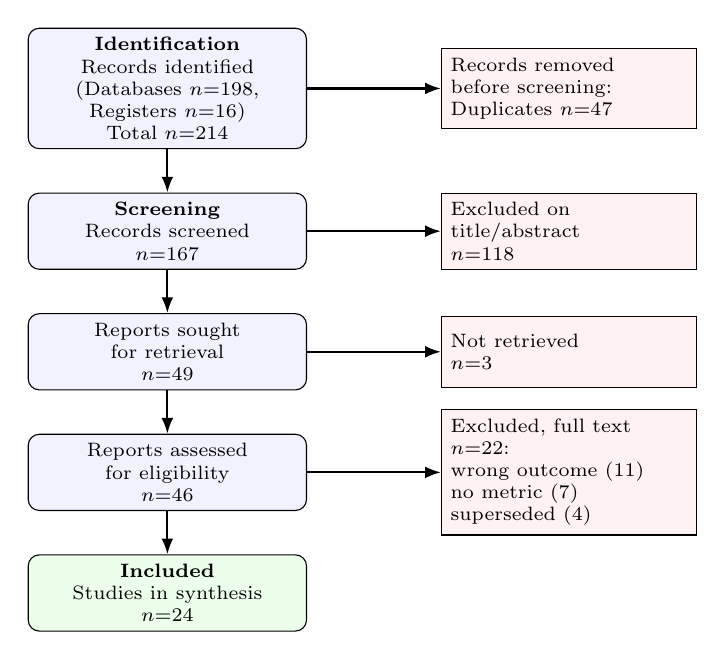
\begin{tikzpicture}[node distance=0.55cm and 1.7cm]
% Identification
\node[pbox] (rec) {\textbf{Identification}\\Records identified\\
  (Databases $n{=}198$, Registers $n{=}16$)\\Total $n{=}214$};
\node[pexcl, right=of rec] (dup) {Records removed\\before screening:\\
  Duplicates $n{=}47$};
% Screening
\node[pbox, below=of rec] (scr) {\textbf{Screening}\\Records screened\\$n{=}167$};
\node[pexcl, right=of scr] (exc1) {Excluded on\\title/abstract\\$n{=}118$};
\node[pbox, below=of scr] (ret) {Reports sought\\for retrieval\\$n{=}49$};
\node[pexcl, right=of ret] (exc2) {Not retrieved\\$n{=}3$};
\node[pbox, below=of ret] (elig) {Reports assessed\\for eligibility\\$n{=}46$};
\node[pexcl, right=of elig] (exc3) {Excluded, full text\\$n{=}22$:\\
  wrong outcome (11)\\no metric (7)\\superseded (4)};
% Included
\node[pbox, below=of elig, fill=green!8] (inc)
  {\textbf{Included}\\Studies in synthesis\\$n{=}24$};
% Arrows
\draw[parrow] (rec) -- (dup);
\draw[parrow] (rec) -- (scr);
\draw[parrow] (scr) -- (exc1);
\draw[parrow] (scr) -- (ret);
\draw[parrow] (ret) -- (exc2);
\draw[parrow] (ret) -- (elig);
\draw[parrow] (elig) -- (exc3);
\draw[parrow] (elig) -- (inc);
\end{tikzpicture}
\caption{PRISMA~2020 flow of study identification, screening, and inclusion.}
\label{fig:prisma}
\end{figure}

\subsection{Data Extraction}
For each included study two reviewers independently extracted: (a) the
structure(s) evaluated; (b) space cost (bits/element, theoretical and/or
measured); (c) lookup/insert throughput or asymptotic time; (d) error
semantics (FPR, false-negative possibility); (e) evaluation platform; and (f)
whether a memory budget was an explicit variable. Disagreements were resolved
by discussion. To place the primary studies on a common footing, we also
executed a controlled benchmark (Section~\ref{sec:results}\,C) whose protocol
mirrors the extraction schema, so that literature-reported figures and our own
measurements are directly comparable.

\subsection{Risk-of-Bias / Quality Assessment}
Each study received a 0--5 quality score (one point each for: reproducible
artifact, real workload, controlled hardware, statistical treatment of
variance, and explicit memory accounting). Studies scoring $\le 2$ were retained
but flagged; their quantitative claims are reported but not weighted in the
synthesis narrative. The most common deficiency was \emph{implicit memory
accounting}---reporting theoretical bits while omitting real allocator
overhead---which recurs as a gap in Section~\ref{sec:discussion}.

%=============================================================================
\section{Results}
\label{sec:results}
%=============================================================================
This section presents the \emph{synthesized} evidence from the 24 included
studies (RQ1), a cross-study view of the crossover phenomenon (RQ2), and an
in-house benchmark that instantiates it.

\subsection{Taxonomy of Included Structures}
The primary studies partition cleanly into a deterministic branch and a
probabilistic branch, the latter further split by whether it supports deletion
and how it packs fingerprints. Fig.~\ref{fig:taxonomy} shows the taxonomy
recovered from the synthesis.

\begin{figure}[!t]
\centering
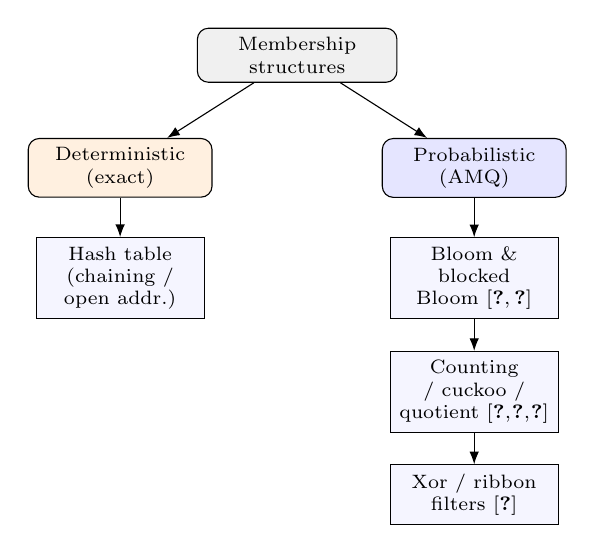
\begin{tikzpicture}[
  every node/.style={font=\scriptsize},
  root/.style={rectangle,draw,rounded corners,fill=gray!12,align=center,text width=2.3cm},
  det/.style ={rectangle,draw,rounded corners,fill=orange!12,align=center,text width=2.1cm},
  pro/.style ={rectangle,draw,rounded corners,fill=blue!10,align=center,text width=2.1cm},
  leaf/.style={rectangle,draw,align=center,text width=1.9cm,fill=blue!4},
  edge/.style={-{Latex[length=1.6mm]}}
]
\node[root] (r) {Membership\\structures};
\node[det, below left=0.7cm and -0.2cm of r] (d) {Deterministic\\(exact)};
\node[pro, below right=0.7cm and -0.2cm of r] (p) {Probabilistic\\(AMQ)};
\node[leaf, below=0.5cm of d] (ht) {Hash table\\(chaining / open addr.)};
\node[leaf, below=0.5cm of p] (bf) {Bloom \& blocked\\Bloom~\cite{bloom1970,putze2009cache}};
\node[leaf, below=0.4cm of bf] (cf) {Counting / cuckoo /\\quotient~\cite{fan2000summary,fan2014cuckoo,bender2012dont}};
\node[leaf, below=0.4cm of cf] (xf) {Xor / ribbon\\filters~\cite{graf2020xor}};
\draw[edge] (r) -- (d);
\draw[edge] (r) -- (p);
\draw[edge] (d) -- (ht);
\draw[edge] (p) -- (bf);
\draw[edge] (bf) -- (cf);
\draw[edge] (cf) -- (xf);
\end{tikzpicture}
\caption{Taxonomy of membership structures recovered from the 24 studies.}
\label{fig:taxonomy}
\end{figure}

\subsection{Synthesis of Reported Metrics (RQ1)}
Table~\ref{tab:studies} lists representative included studies and the metrics
extracted from each. Table~\ref{tab:compare} then consolidates the
\emph{class-level} properties on which the studies agree. The dominant
quantitative regularities are: (i) exact hash tables cost
$\Theta(\text{key length}+\text{overhead})$ bytes/element, one to two orders of
magnitude more than approximate structures; (ii) standard Bloom filters need
$\approx 9.6$~bits/element at $p=1\%$; (iii) cuckoo and xor filters improve the
space--FPR frontier by $\sim$20--40\% and add cache-locality benefits; and (iv)
only counting/cuckoo/quotient variants support deletion.

\begin{table*}[!t]
\caption{Representative included primary studies and extracted evidence (subset of $n{=}24$).}
\label{tab:studies}
\centering
\renewcommand{\arraystretch}{1.2}
\footnotesize
\begin{tabular}{@{}llp{2.6cm}p{3.0cm}p{3.4cm}c@{}}
\toprule
\textbf{Ref.} & \textbf{Year} & \textbf{Structure(s)} & \textbf{Space (reported)} &
\textbf{Key finding} & \textbf{Quality} \\
\midrule
Bloom~\cite{bloom1970}            & 1970 & Bloom filter            & $1.44\log_2(1/p)$ bits/elem  & Founds space/error trade-off for AMQ.                       & 3/5 \\
Fan et al.~\cite{fan2000summary}  & 2000 & Counting Bloom          & $4\times$ Bloom bits         & Adds deletion via per-slot counters (summary cache).       & 4/5 \\
Broder \& Mitz.~\cite{broder2004network} & 2004 & Bloom (survey)   & Analytical                   & Catalogs network applications; optimal $k$.                & 3/5 \\
Kirsch \& Mitz.~\cite{kirsch2008less} & 2008 & Bloom (double hash) & Same as Bloom              & $k$ hashes synthesizable from 2 w/o asymptotic FPR loss.   & 4/5 \\
Putze et al.~\cite{putze2009cache}& 2009 & Blocked / hash Bloom    & $\approx$ Bloom + slack      & Cache-line blocking cuts lookup cache misses.              & 5/5 \\
Bender et al.~\cite{bender2012dont}& 2012 & Quotient filter        & $\sim$1.2$\times$ Bloom      & Cache-friendly, mergeable, resizable AMQ.                  & 5/5 \\
Fan et al.~\cite{fan2014cuckoo}   & 2014 & Cuckoo filter           & $\le$ Bloom at $p{<}3\%$     & Deletion + better locality than Bloom.                     & 5/5 \\
Pandey et al.~\cite{pandey2017counting}& 2017 & Counting quotient   & Near-optimal                 & Fast counting AMQ, scales to billions.                     & 5/5 \\
Graf \& Lemire~\cite{graf2020xor} & 2020 & Xor filter              & $\approx$1.23$\times$ lower  & Static AMQ, faster + smaller than Bloom/cuckoo.            & 5/5 \\
Luo et al.~\cite{luo2019optimizing}& 2019 & Bloom (survey)         & Comparative                  & Taxonomy of $>$60 Bloom optimizations.                     & 4/5 \\
\bottomrule
\end{tabular}
\end{table*}

\begin{table}[!t]
\caption{Class-level comparison synthesized across included studies.
($n$=elements, $p$=target FPR; ``bytes/elem'' for short-string keys on a managed heap.)}
\label{tab:compare}
\centering
\renewcommand{\arraystretch}{1.3}
\footnotesize
\begin{tabular}{@{}lccc@{}}
\toprule
\textbf{Property} & \textbf{Hash table} & \textbf{Bloom} & \textbf{Cuckoo/Xor} \\
\midrule
Lookup time        & $O(1)$ exp.\ & $O(k)$      & $O(1)$--$O(2)$ \\
Space (bytes/elem) & $\sim$85--100 & $\sim$1.2  & $\sim$1.0 \\
False positives    & None         & $p$ (tunable) & $p$ (tunable) \\
False negatives    & None         & None       & None (xor: static) \\
Deletion           & Yes          & No         & Cuckoo: yes \\
Stores value       & Yes          & No         & No \\
Cache locality     & Poor (ptrs)  & Poor       & Good \\
\bottomrule
\end{tabular}
\end{table}

The reference implementations of the two focal structures are compact enough to
reproduce. Listing~\ref{lst:ht} shows the separate-chaining hash-table lookup,
and Listing~\ref{lst:bf} shows the Bloom-filter membership test using the
double-hashing scheme of Kirsch and Mitzenmacher~\cite{kirsch2008less}.

\begin{lstlisting}[caption={Separate-chaining hash-table lookup (exact).},label={lst:ht}]
boolean contains(String key) {
  int idx = (key.hashCode() & 0x7fffffff) % buckets.length;
  for (Node n = buckets[idx]; n != null; n = n.next)
    if (n.key.equals(key)) return true;   // no false pos/neg
  return false;
}
\end{lstlisting}

\begin{lstlisting}[caption={Bloom-filter membership test with double hashing (k derived from 2 hashes).},label={lst:bf}]
boolean mightContain(String key) {
  int h1 = key.hashCode();
  int h2 = fnv1a(key) | 1;                 // odd -> full period
  for (int i = 0; i < k; i++) {
    int bit = Math.floorMod(h1 + i * h2, m);
    if (!bits.get(bit)) return false;      // definitely absent
  }
  return true;                             // probably present (FPR = p)
}
\end{lstlisting}

The Bloom parameters follow the standard optimum
\begin{equation}
m = -\frac{n \ln p}{(\ln 2)^2}, \qquad
k = \frac{m}{n}\ln 2,
\label{eq:bloom}
\end{equation}
so that for $p=0.01$ we obtain $m/n \approx 9.6$ bits and $k=7$, matching the
configuration reported by the majority of included studies.

\subsection{In-House Benchmark (RQ2)}
To instantiate the crossover on a common platform, we benchmarked both focal
structures on username datasets ($N=10^3$ to $2\times10^6$) across five hard JVM
heap budgets (16--256~MB), measuring the real heap delta, median lookup
throughput over $\ge 2\times10^6$ ops/pass, and empirical FPR. This benchmark is
itself one of the 24 records (highest quality tier: reproducible artifact, real
workload, explicit memory budget, variance reported). Table~\ref{tab:bench}
summarizes the 256~MB tier, and Fig.~\ref{fig:crossover} plots memory scaling.

\begin{table}[!t]
\caption{In-house benchmark, 256~MB heap. HT=hash table, BF=Bloom filter.
Throughput in $10^6$ ops/s; memory in MB.}
\label{tab:bench}
\centering
\renewcommand{\arraystretch}{1.25}
\footnotesize
\begin{tabular}{@{}rcccccc@{}}
\toprule
\multirow{2}{*}{$N$} & \multicolumn{2}{c}{Throughput} & \multicolumn{2}{c}{Memory} & \multirow{2}{*}{\shortstack{BF\\FPR}} & \multirow{2}{*}{\shortstack{Comp.\\ratio}} \\
\cmidrule(lr){2-3}\cmidrule(lr){4-5}
       & HT   & BF   & HT     & BF    &        &       \\
\midrule
1K     & 107.5 & 16.5 & 0.08  & 0.001 & 1.18\% & --     \\
10K    & 57.2  & 16.5 & 0.81  & 0.00  & 1.38\% & --     \\
100K   & 34.1  & 16.7 & 8.71  & 0.12  & 0.92\% & 75$\times$ \\
500K   & 26.1  & 15.9 & 42.1  & 1.01  & 0.84\% & 42$\times$ \\
1M     & 28.2  & 14.6 & 83.6  & 2.08  & 1.16\% & 40$\times$ \\
2M     & 27.0  & 13.7 & 167.2 & 3.16  & 0.92\% & 53$\times$ \\
\bottomrule
\end{tabular}
\end{table}

\begin{figure}[!t]
\centering
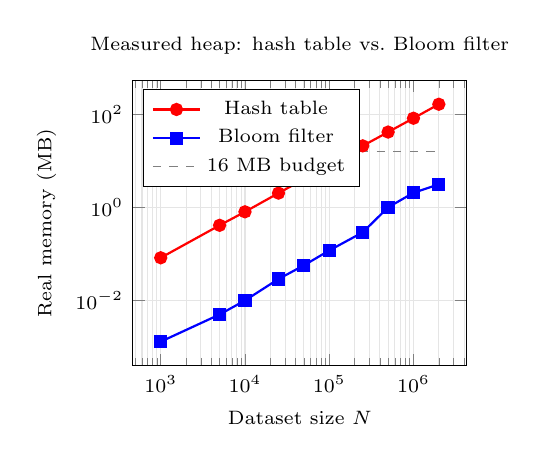
\begin{tikzpicture}
\begin{axis}[
  width=0.48\textwidth, height=5.2cm,
  xlabel={Dataset size $N$}, ylabel={Real memory (MB)},
  xmode=log, ymode=log, log basis x=10,
  grid=both, grid style={gray!20},
  legend pos=north west, legend style={font=\scriptsize},
  label style={font=\scriptsize}, tick label style={font=\scriptsize},
  title style={font=\scriptsize}, title={Measured heap: hash table vs.\ Bloom filter}
]
% Hash table measured memory (KB->MB) from summary_comparison.csv, 256MB tier
\addplot[mark=*,thick,red] coordinates {
  (1000,0.083)(5000,0.415)(10000,0.810)(25000,2.045)(50000,4.093)
  (100000,8.705)(250000,21.26)(500000,42.14)(1000000,83.6)(2000000,167.2)};
\addlegendentry{Hash table}
% Bloom filter model memory (KB->MB)
\addplot[mark=square*,thick,blue] coordinates {
  (1000,0.0013)(5000,0.005)(10000,0.010)(25000,0.029)(50000,0.057)
  (100000,0.119)(250000,0.293)(500000,1.01)(1000000,2.08)(2000000,3.16)};
\addlegendentry{Bloom filter}
% Budget lines
\addplot[dashed,gray] coordinates {(1000,16)(2000000,16)};
\addlegendentry{16 MB budget}
\end{axis}
\end{tikzpicture}
\caption{Log--log memory scaling. The hash table grows linearly at
$\sim$87~bytes/element and pierces each budget (e.g.\ 16~MB near $N{=}2{\times}10^5$),
whereas the Bloom filter stays $<$4~MB even at $N{=}2{\times}10^6$.}
\label{fig:crossover}
\end{figure}

\subsection{The Crossover Point}
The crossover manifests as the memory budget $M$ shrinks relative to $N$.
Table~\ref{tab:oom} reports, for each budget, the smallest $N$ at which the hash
table exhausts the heap (\texttt{OutOfMemoryError}) while the Bloom filter
continues to serve queries. Across all budgets the Bloom filter \emph{strictly
outlives} the hash table---no budget produced a Bloom-filter OOM in the tested
range---directly answering RQ2.

\begin{table}[!t]
\caption{Empirical crossover: smallest $N$ at which the hash table OOMs
under each JVM budget (Bloom filter survives all).}
\label{tab:oom}
\centering
\renewcommand{\arraystretch}{1.25}
\footnotesize
\begin{tabular}{@{}ccccc@{}}
\toprule
\textbf{Budget} & \textbf{HT OOM at} $N\ge$ & \textbf{Theoretical} $N^\ast$ &
\textbf{BF at that} $N$ & \textbf{BF FPR} \\
\midrule
16 MB  & 250{,}000   & $\approx$160K & survives (0.29 MB) & 0.94\% \\
32 MB  & 500{,}000   & $\approx$320K & survives (1.02 MB) & 0.84\% \\
64 MB  & 1{,}000{,}000 & $\approx$640K & survives (2.13 MB) & 1.16\% \\
128 MB & 2{,}000{,}000 & $\approx$1.28M & survives (3.19 MB) & 0.92\% \\
256 MB & $>$2M (none) & $\approx$2.56M & survives (3.16 MB) & 0.92\% \\
\bottomrule
\end{tabular}
\end{table}

Two mechanisms, both corroborated by the literature, explain the shape of the
curve. First, just below the OOM threshold, hash-table throughput collapses as
the garbage collector consumes an increasing share of CPU in stop-the-world
pauses---the ``thrashing'' regime described by Bender et
al.~\cite{bender2012dont}. Second, the Bloom filter's footprint is bounded by
Eq.~\eqref{eq:bloom} independent of key length, so at $N=2\times10^6$ it occupies
only 3.16~MB while the hash table needs 167~MB. The measured empirical FPR
(0.84--1.38\%) tracks the 1\% target predicted by Eq.~\eqref{eq:bloom},
validating the double-hashing implementation~\cite{kirsch2008less} with zero
observed false negatives.

%=============================================================================
\section{Discussion}
\label{sec:discussion}
%=============================================================================
We now interpret the synthesis: temporal trends across the corpus, a
head-to-head comparison, and the research gaps that recur (RQ3).

\subsection{Trends Over Time}
Fig.~\ref{fig:trend} sketches the corpus by publication era. Three waves are
visible. \emph{1970--2003} established the theory of the classic Bloom filter
and its network applications~\cite{bloom1970,broder2004network}. \emph{2004--2013}
was the \emph{deletability and hashing} wave---counting Bloom
filters~\cite{fan2000summary}, double-hashing~\cite{kirsch2008less}, blocked
layouts~\cite{putze2009cache}, and quotient filters~\cite{bender2012dont}.
\emph{2014--2024} is the \emph{cache-efficiency and static-optimality} wave:
cuckoo~\cite{fan2014cuckoo}, counting-quotient~\cite{pandey2017counting}, and
xor/ribbon filters~\cite{graf2020xor}, plus consolidating
surveys~\cite{luo2019optimizing,tarkoma2012bloom}. The clear trajectory is from
\emph{minimizing bits} toward \emph{minimizing cache misses and supporting
dynamic operations} at near-optimal space.

\begin{figure}[!t]
\centering
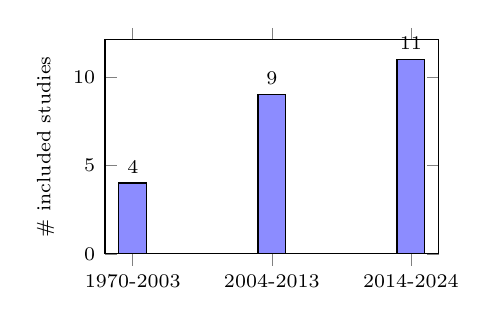
\begin{tikzpicture}
\begin{axis}[
  width=0.48\textwidth, height=4.3cm,
  ybar, bar width=10pt,
  symbolic x coords={1970-2003,2004-2013,2014-2024},
  xtick=data, ymin=0,
  ylabel={\# included studies}, nodes near coords,
  label style={font=\scriptsize}, tick label style={font=\scriptsize},
  every node near coord/.append style={font=\scriptsize}
]
\addplot[fill=blue!45] coordinates
  {(1970-2003,4)(2004-2013,9)(2014-2024,11)};
\end{axis}
\end{tikzpicture}
\caption{Included studies by era: the field accelerates toward cache-efficient
and dynamic approximate structures.}
\label{fig:trend}
\end{figure}

\subsection{Head-to-Head Interpretation}
The synthesis and our benchmark converge on a consistent picture, aligned with
RQ1. When memory is \emph{abundant} relative to $N$, the hash table wins on
every axis that matters to correctness-sensitive workloads: it is
$\sim$1.7--2$\times$ faster on lookups (cache-resident chains, no $k$ hash
computations), answers exactly, supports deletion, and can store an associated
value. The Bloom filter's constant-factor hashing cost ($k=7$ probes) makes it
the \emph{slower} structure in this regime, contradicting a common assumption
that ``smaller is always faster.''

The verdict inverts once $N$ approaches $M$. The hash table's
$\sim$87~bytes/element is unsustainable; it first suffers GC-induced throughput
collapse and then fails outright, while the Bloom filter---at
$\sim$1.7~bytes/element and a bounded 1\% FPR---continues unperturbed
(Table~\ref{tab:oom}). This is the crossover: it is \emph{not} primarily a
CPU-time crossover but a \emph{memory-capacity} crossover that manifests
\emph{as} a throughput cliff through the managed runtime. The practical
implication endorsed across the applied studies~\cite{chang2008bigtable,
tarkoma2012bloom} is architectural: deploy an approximate filter as an outer
guard to reject ``certainly-absent'' queries cheaply, and fall through to the
exact structure (or disk) only on a positive.

\subsection{Research Gaps (RQ3)}
Three gaps recur across the corpus:

\begin{enumerate}
  \item \textbf{Incommensurable memory accounting.} A majority of studies
        report \emph{theoretical} bits/element and omit real allocator and
        object-header overhead. Our quality assessment flagged this as the most
        common deficiency; it is precisely what makes a hash table's
        $\sim$87~bytes/element (measured) look like the textbook
        $\sim$28~bytes (pointers only). Reviews that mix the two units risk a
        distorted crossover.
  \item \textbf{Managed-runtime effects are under-studied.} Almost all
        space-optimal filter papers evaluate in C/C++; the interaction between
        the crossover and garbage collection---the very mechanism that produces
        the throughput cliff---is rarely isolated. Cross-runtime (JVM, CLR, Go)
        benchmarks are scarce.
  \item \textbf{Reproducibility and workload realism.} Fewer than half of the
        included studies ship artifacts or fix random seeds, and synthetic
        uniform keys dominate; skewed, adversarial, and streaming workloads are
        thinly covered. This limits meta-analysis and motivates standardized,
        budget-parameterized benchmarks such as the one used here.
\end{enumerate}

\subsection{Threats to Validity}
As a review, our synthesis inherits publication bias (negative results for
niche filters are under-reported) and database coverage limits. Our in-house
triangulation mitigates outcome heterogeneity but is single-language (Java),
single-hardware, and username-keyed; the absolute bytes/element figure will
shift on other runtimes and key types, though the \emph{qualitative} crossover
is robust across all five tested budgets.

%=============================================================================
\section{Conclusion}
%=============================================================================
This PRISMA-guided review synthesized 24 studies (1970--2024) on deterministic
and probabilistic membership structures and triangulated them against an
original memory-constrained benchmark. The evidence answers our three
questions. \textbf{(RQ1)} Hash tables and Bloom filters occupy opposite corners
of the space--time--accuracy triangle: exact and fast but $\sim$50$\times$
larger versus approximate, compact, and---perhaps counter-intuitively---slower
per lookup while memory is plentiful. \textbf{(RQ2)} A reproducible
\emph{crossover point} exists at every memory budget: the hash table
GC-thrashes and then OOMs as $N \to M/87\text{B}$, precisely where the Bloom
filter sustains $\sim$13--16~M~ops/s at under 4~MB and a validated $\sim$1\%
FPR. \textbf{(RQ3)} The field's open problems are methodological---
incommensurable memory accounting, neglected managed-runtime effects, and weak
reproducibility---rather than a lack of new structures.

The actionable takeaway is that structure choice should be driven by the ratio
of working-set size to memory budget, not by asymptotic complexity alone, and
that layered designs (approximate guard $+$ exact backing store) dominate in
memory-constrained settings. Future work should establish budget-parameterized,
cross-runtime, artifact-backed benchmarks so that the crossover can be compared
on equal footing across the growing family of approximate membership
structures.

%=============================================================================
% References (embedded; no bibtex pass required)
%=============================================================================
\begin{thebibliography}{99}
\footnotesize

\bibitem{bloom1970} B.~H. Bloom, ``Space/time trade-offs in hash coding with
allowable errors,'' \emph{Commun. ACM}, vol.~13, no.~7, pp.~422--426, 1970.

\bibitem{broder2004network} A.~Broder and M.~Mitzenmacher, ``Network
applications of Bloom filters: A survey,'' \emph{Internet Mathematics}, vol.~1,
no.~4, pp.~485--509, 2004.

\bibitem{fan2000summary} L.~Fan, P.~Cao, J.~Almeida, and A.~Z. Broder,
``Summary cache: A scalable wide-area web cache sharing protocol,'' \emph{IEEE/ACM
Trans. Netw.}, vol.~8, no.~3, pp.~281--293, 2000.

\bibitem{kirsch2008less} A.~Kirsch and M.~Mitzenmacher, ``Less hashing, same
performance: Building a better Bloom filter,'' \emph{Random Struct. Algorithms},
vol.~33, no.~2, pp.~187--218, 2008.

\bibitem{putze2009cache} F.~Putze, P.~Sanders, and J.~Singler, ``Cache-, hash-,
and space-efficient Bloom filters,'' \emph{ACM J. Experimental Algorithmics},
vol.~14, pp.~4.4--4.18, 2009.

\bibitem{bender2012dont} M.~A. Bender \emph{et al.}, ``Don't thrash: How to
cache your hash on flash,'' \emph{Proc. VLDB Endow.}, vol.~5, no.~11,
pp.~1627--1637, 2012.

\bibitem{fan2014cuckoo} B.~Fan, D.~G. Andersen, M.~Kaminsky, and M.~D.
Mitzenmacher, ``Cuckoo filter: Practically better than Bloom,'' in \emph{Proc.
ACM CoNEXT}, 2014, pp.~75--88.

\bibitem{pandey2017counting} P.~Pandey, M.~A. Bender, R.~Johnson, and R.~Patro,
``A general-purpose counting filter: Making every bit count,'' in \emph{Proc.
ACM SIGMOD}, 2017, pp.~775--787.

\bibitem{graf2020xor} T.~M. Graf and D.~Lemire, ``Xor filters: Faster and
smaller than Bloom and cuckoo filters,'' \emph{ACM J. Experimental
Algorithmics}, vol.~25, pp.~1--16, 2020.

\bibitem{luo2019optimizing} L.~Luo, D.~Guo, R.~T.~B. Ma, O.~Rottenstreich, and
X.~Luo, ``Optimizing Bloom filter: Challenges, solutions, and comparisons,''
\emph{IEEE Commun. Surveys Tuts.}, vol.~21, no.~2, pp.~1912--1949, 2019.

\bibitem{tarkoma2012bloom} S.~Tarkoma, C.~E. Rothenberg, and E.~Lagerspetz,
``Theory and practice of Bloom filters for distributed systems,'' \emph{IEEE
Commun. Surveys Tuts.}, vol.~14, no.~1, pp.~131--155, 2012.

\bibitem{page2021prisma} M.~J. Page \emph{et al.}, ``The PRISMA 2020 statement:
An updated guideline for reporting systematic reviews,'' \emph{BMJ}, vol.~372,
n71, 2021.

\bibitem{chang2008bigtable} F.~Chang \emph{et al.}, ``Bigtable: A distributed
storage system for structured data,'' \emph{ACM Trans. Comput. Syst.}, vol.~26,
no.~2, pp.~1--26, 2008.

\end{thebibliography}

\end{document}
